
\subsection{Red de una universidad}
Este experimento se realizó sobre la red Wi-Fi de acceso público \textit{EXACTAS-UBA}, en la zona de aulas del pabellón 1 de la FCEyN, realizando una captura de 45 minutos a las 19 horas.
Suponemos que esta red es usada por alumnos y profesores durante las clases.

Durante la medición vació manualmente la caché ARP de un host.

\subsubsection{Fuente S}

Mediante las herramientas ya presentadas obtuvimos los siguientes resultados
\begin{itemize}
 \item $38507$ paquetes unicasts
 \item $103$ paquetes broadcasts
 \item $38610$ paquetes en total
 \item $H(S) = 0.02665$
\end{itemize}

\begin{figure}[H]
   \centering
       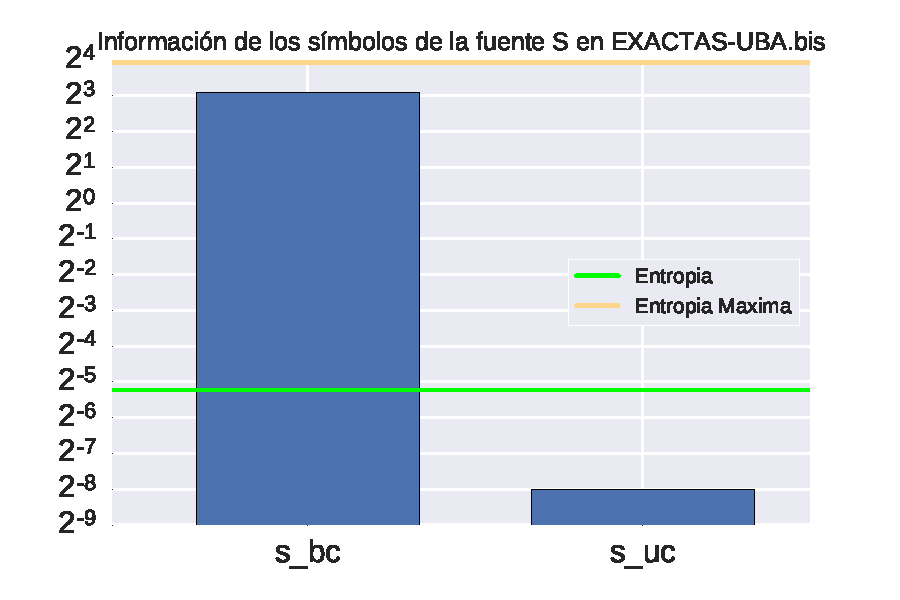
\includegraphics[page=1,width=.70\textwidth]{../img/barras-EXACTAS-UBA-bis}
 \caption{Entropía de la red}
 \label{fig:barras-exactas}
\end{figure}

Las mediciones de la figura \ref{fig:barras-exactas} se corresponden con el uso de la red puramente para acceder a servidores externos que se esperaría de los alumnos durante una clase.
Efectivamente, analizando el tráfico comprobamos que el 99.7\% de los paquetes tienen como MAC de fuente o destino al default gateway.

 \subsubsection{Grafo de conectividad de la red}
 Grafo de conectividad de la red para visualizar el comportamiento de la misma.


\begin{figure}[H]
   \centering
       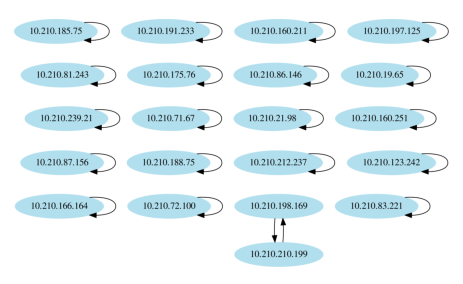
\includegraphics[page=1,height=8cm ,width=1.08\textwidth]{../img/red-EXACTAS-UBA-bis}
 \caption{Grafo de conectividad}
 \label{fig:grafo-exactas}
\end{figure}

Al graficar el tráfico ARP sensado vemos que aparte de la petición por la MAC del gateway que se generó al vaciar la caché el resto del tráfico se compone enteramente de gratuitous ARPs.
Esto se puede deber a que todos los hosts de la red ya estaban conectados cuando se inició la captura, y ya tenían en su caché la MAC del gateway.


\subsubsection{Información y nodos distinguidos}

Para esta sección reutilizamos la herramienta presentada en el ejercicio 2 con el objetivo de analizar la presencia de nodos distinguidos de la fuente. \\

\begin{figure}[H]
    \centering
    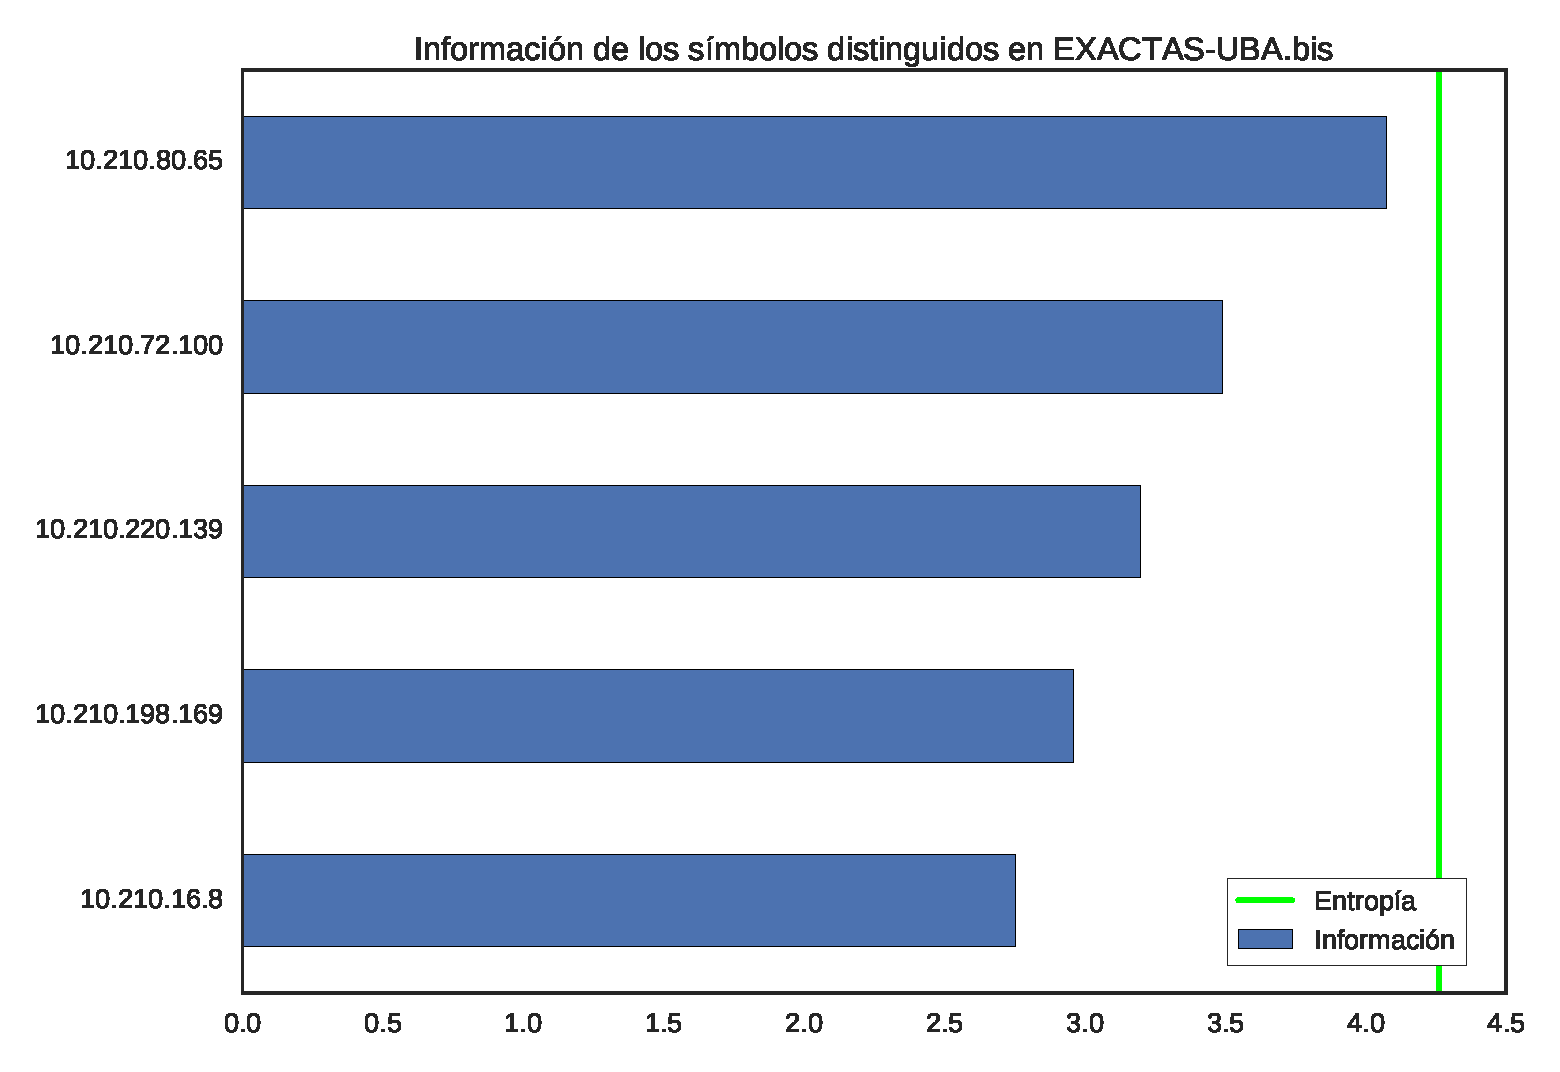
\includegraphics[page=1, height=6.55cm ,width=\textwidth]{../img/distinguidos-EXACTAS-UBA-bis}
    \caption{Nodos distinguidos}
    \label{fig:distinguidos-exactas}
\end{figure}

Como se puede observar en la figura \ref{fig:distinguidos-exactas}, la gran cantidad de gratuitous ARPs no nos permite encontrar conclusivamente el default gateway.
